\begin{name}
	{\tenchude}{\tendethi}{LỚP TOÁN THẦY PHÁT}{\thoigian}
\end{name}
\setcounter{ex}{0}\setcounter{bt}{0}
\Opensolutionfile{ans}[ans/ans-2-TT-10-ChuyenThaiBinh-23-L3]
\begin{ex}%[Đề thi thử TN THPT Lần 3, THPT Chuyên Thái Bình năm 2023]%[BCTuan, dự án 12EX6-2023]%[2H3Y1-1]%Câu 1
	Trong KG $Oxyz$, cho $\overrightarrow {a}=-\overrightarrow{i}+2\overrightarrow {j}-3\overrightarrow{k}$. Tọa độ của véc-tơ $\overrightarrow{a}$ là
	\choice
	{$(2;-1;-3)$}
	{$(-3;2;1)$}
	{$(2;-3;-1)$}
	{\True $(-1;2;-3)$}
	\loigiai{
		Ta có $\overrightarrow{a}=(-1;2;-3)$.
	}
\end{ex}

\begin{ex}%[Đề thi thử TN THPT Lần 3, THPT Chuyên Thái Bình năm 2023]%[BCTuan, dự án 12EX6-2023]%[2D1Y2-2]%Câu 2
	Cho hàm số $f(x)$ có bảng biến thiên như hình vẽ
	\begin{center}
		
\begin{tikzpicture}
			\tkzTabInit[lgt=1.2,espcl=2.5,deltacl=0.6,nocadre=false]
			{$x$/0.8, $y'$/0.8, $y$/2.5}
			{$-\infty$,$1$,$2$,$+\infty$}
			\tkzTabLine{ ,-,0,+,0,-, }
			\tkzTabVar{+/$4$,-/$-2$,+/$3$,-/$-3$}
		\end{tikzpicture}
	\end{center}
	Khẳng định nào sau đây đúng?
	\choice
	{\True Giá trị cực đại của hàm số là $y_{\text{CĐ}}=3$}
	{Giá trị cực đại của hàm số là $y_{\text{CĐ}}=4$}
	{Giá trị cực tiểu của hàm số là $y_{\text{CT}}=-3$}
	{Giá trị cực tiểu của hàm số là $y_{\text{CT}}=1$}
	\loigiai{
Dựa vào bảng biến thiên hàm số, giá trị cực đại của hàm số là $y_{\text{CĐ}}=3$.
	}
\end{ex}

\begin{ex}%[Đề thi thử TN THPT Lần 3, THPT Chuyên Thái Bình năm 2023]%[BCTuan, dự án 12EX6-2023]%[2D1Y5-1]%Câu 3
\immini
{
		Hàm số nào dưới đây có đồ thị như đường cong trong hình vẽ bên?
	\choice
	{$y=x^3-2x$}
	{$y=2x^2-x^4$}
	{$y=-x^3+3x^2$}
	{\True $y=x^4-2x^2$}
}
{
	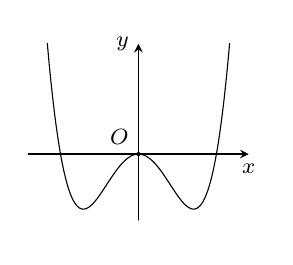
\begin{tikzpicture}[scale=0.7, font=\footnotesize, line join=round, line cap=round, >=stealth]
		\draw [->] (-2,0)--(2,0)node[below]{\footnotesize $x$};
		\draw [->] (0,-1.2)--(0,2)node[left]{\footnotesize $y$};
		\draw [fill=black,draw=black] (0,0) circle (1pt)node[above left] {\footnotesize $O$};
		\clip(-2,-1.5) rectangle (2,2);
		\draw[smooth,samples=100,domain=-2:2]  plot(\x,{(\x)^4-2*(\x)^2});
	\end{tikzpicture}
}
	\loigiai{
		Hình vẽ trên là đồ thị của hàm số bậc bốn trùng phương $y=ax^4+bx^2+c$, với hệ số $a>0$ nên chọn đáp án $y=x^4-2x^2$.
	}
\end{ex}

\begin{ex}%[Đề thi thử TN THPT Lần 3, THPT Chuyên Thái Bình năm 2023]%[BCTuan, dự án 12EX6-2023]%[2D2Y2-1]%Câu 4
	Tìm tập xác định $\mathscr{D}$ của hàm số $y=(x^2-x-2)^{-5}$.
	\choice
	{$\mathscr{D}=\mathbb{R}$}
	{$\mathscr{D}=(0;+\infty)$}
	{$\mathscr{D}=(-\infty ;-1)\cup(2;+\infty)$}
	{\True $\mathscr{D}=\mathbb{R}\setminus \{-1;2\}$}
	\loigiai{
		Vì $-5$ là số nguyên âm nên
	hàm số xác định khi và chỉ khi $x^2-x-2\ne 0\Leftrightarrow \heva{&
			x\ne-1\\&
			x\ne 2.}$\\
		Vậy $\mathscr{D}=\mathbb{R}\setminus \{-1;2\}$.}
\end{ex}

\begin{ex}%[Đề thi thử TN THPT Lần 3, THPT Chuyên Thái Bình năm 2023]%[BCTuan, dự án 12EX6-2023]%[2D3Y1-1]%Câu 5
	Tìm họ nguyên hàm của hàm số $f(x)=\sin 3x$.
	\choice
	{$-\cos 3x+C$}
	{\True $-\dfrac{1}{3}\cos 3x+C$}
	{$\cos 3x+C$}
	{$\dfrac{1}{3}\cos 3x+C$}
	\loigiai{
		Ta có $\displaystyle\int \sin 3x\mathrm{\,d}x=-\dfrac{1}{3}\cos 3x+C$.}
\end{ex}

\begin{ex}%[Đề thi thử TN THPT Lần 3, THPT Chuyên Thái Bình năm 2023]%[BCTuan, dự án 12EX6-2023]%[1D3Y3-3]%Câu 6
	Cho cấp số nhân $(u_n)$ có số hạng đầu $u_1=3$ và công bội $q=2$. Số hạng thứ năm của cấp số nhân là
	\choice
	{$u_5=96$}
	{$u_5=32$}
	{\True $u_5=48$}
	{$u_5=24$}
	\loigiai{
		Ta có $u_5=u_1\cdot q^4=3\cdot 2^4=48$.}
\end{ex}

\begin{ex}%[Đề thi thử TN THPT Lần 3, THPT Chuyên Thái Bình năm 2023]%[BCTuan, dự án 12EX6-2023]%[2H1B3-2]
	Cho khối hộp chữ nhật $ABCD.A'B'C'D'$ có $AA'=a$, $AB=3a$, $AC=5a$. Thể tích khối hộp $ABCD.A'B'C'D'$ là
	\choice
	{\True $12a^3$}
	{$4a^3$}
	{$15a^3$}
	{$5a^3$}
	\loigiai{
		\immini{
			Ta có $AD=\sqrt{AC^2-AB^2}=4a$.\\
			Thể tích khối hộp $ABCD.A'B'C'D'$ là $V=AB\cdot AD\cdot AA'=3a\cdot 4a\cdot a=12a^3$.
		}{
			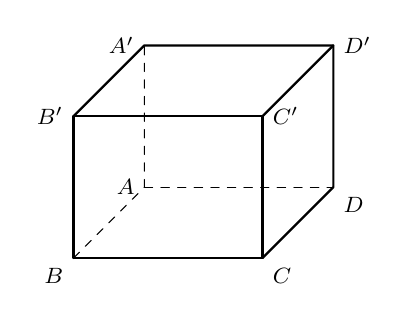
\begin{tikzpicture}[scale=0.6, font=\footnotesize, line join=round, line cap=round, >=stealth]
				\draw[thick] (0,0)node[below left]{$B$}--++(4,0)node[below right]{$C$}--++(0,3)node[right]{$C'$}--++(-4,0)node[left]{$B'$}--++(0,-3);%từ B
				\draw[thick] (4,0)--++(1.5,1.5)node[below right]{$D$}--++(0,3)node[right]{$D'$}--++(-4,0)node[left]{$A'$}--++(-1.5,-1.5);%từ C
				\draw[thick] (4,3)--++(1.5,1.5);%từ C'
				\draw[dashed] (0,0)--++(1.5,1.5)--++(0,3);%từ B
				\draw[dashed] (1.5,1.5)node[left]{$A$}--++(4,0);%từ A
			\end{tikzpicture}
		}
	}
\end{ex}

\begin{ex}%[Đề thi thử TN THPT Lần 3, THPT Chuyên Thái Bình năm 2023]%[BCTuan, dự án 12EX6-2023]%[1D2Y2-1]%Câu 8
	Số tổ hợp chập $3$ của $12$ phần tử là
	\choice
	{$1728$}
	{\True $220$}
	{$1320$}
	{$36$}
	\loigiai{
		Số tổ hợp chập $3$ của $12$ phần tử là $\mathrm{C}_{12}^3=\dfrac{12!}{3!9!}=\dfrac{10\cdot 11\cdot 12}{6}=220$.}
\end{ex}

\begin{ex}%[Đề thi thử TN THPT Lần 3, THPT Chuyên Thái Bình năm 2023]%[BCTuan, dự án 12EX6-2023]%[2H1K3-2] 
	Cho hình chóp $S.ABC$ có đáy $ABC$ là tam giác cân $AB=AC=a$, $\widehat{BAC}=120^\circ$. Các cạnh bên bằng nhau và cùng tạo với mặt phẳng đáy góc $30^\circ$. Thể tích khối chóp $S.ABC$ là
	\choice
	{$\dfrac{3a^3\sqrt{3}}{12}$}
	{$\dfrac{a^3}{4}$}
	{$\dfrac{a^3\sqrt{3}}{4}$}
	{\True $\dfrac{a^3}{12}$}
	\loigiai{
		\immini{Gọi $M$ là trung điểm của $BC$, $H$ là tâm đường tròn ngoại tiếp tam giác $ABC\Rightarrow SH\perp (ABC)$.\\
			Ta có $BC=\sqrt{AB^2+AC^2-2AB\cdot AC\cdot\cos120^\circ}=a\sqrt{3}$.\\
			Và $S_{ABC}=\dfrac{1}{2}AB\cdot AC\cdot\sin120^\circ=\dfrac{a^2\sqrt{3}}{4}$.\\
			Mà $S_{ABC}=\dfrac{AB\cdot BC\cdot CA}{4R}\Rightarrow R=\dfrac{AB\cdot BC\cdot CA}{4S_{ABC}}=a=AH$.\\
			Vì $SH\perp (ABC)$ nên
			$ \left(SA,(ABC)\right)=(SA,AH)=30^\circ$\\
			$\Rightarrow SH=AH\cdot\tan30^\circ=\dfrac{a}{\sqrt{3}}$.\\
			Vậy thể tích khối chóp là
			$$V_{S.ABC}=\dfrac{1}{3}SH\cdot S_{ABC}=\dfrac{a^3}{12}.$$
		}{\begin{tikzpicture}[scale=1, font=\footnotesize, line join=round, line cap=round, >=stealth]
				\path
				(0,0) coordinate (A)
				(5,0) coordinate (C)
				(1,-2) coordinate (B)
				($(B)!0.5!(C)$) coordinate (M)
				($(A)!0.65!(M)$) coordinate (H)
				($(H)+(0,4)$) coordinate (S)
				;
				\draw 
				(S)--(A)--(B)--(C)--(S)--(B)
				;
				\draw[dashed] 
				(A)--(M)
				(S)--(H) (B)--(H)--(C)
				(A)--(C)
				;
				\foreach \p/\g in {A/180/, B/-90, C/-30, H/-100, M/-30, S/90}
				\draw[fill=black] (\p) circle (1pt) node[shift=(\g:3mm)] {$\p$};
				\pic[draw,angle radius=2mm]{right angle = S--H--M};
				\pic[draw,angle radius=2mm]{right angle = A--M--B}
				;
				\pic[draw,angle radius=3mm,fill=gray,opacity=0.3]{angle = H--A--S}
				;
				\pic[draw,angle radius=3mm,fill=gray,opacity=0.3]{angle = S--C--H}
				;
				\pic[draw,angle radius=3mm,fill=gray,opacity=0.3]{angle = H--B--S}
				;
		\end{tikzpicture}}
	}
\end{ex}

\begin{ex}%[Đề thi thử TN THPT Lần 3, THPT Chuyên Thái Bình năm 2023]%[BCTuan, dự án 12EX6-2023]%[2D2Y4-3]%Câu 10
	Trong các hàm số sau, hàm số nào đồng biến trên $\mathbb{R}$?
	\choice
	{$f(x)=\left(\dfrac{\mathrm{e}}{\pi}\right)^x$}
	{$f(x)=\left(\dfrac{1}{\mathrm{e}}\right)^x$}
	{$f(x)=\left(\dfrac{1}{\sqrt{3}}\right)^x$}
	{\True $f(x)=3^x$}
	\loigiai{
		Hàm số mũ $y=a^x$ đồng biến trên $\mathbb{R}$ khi $a > 1$.\\
Vậy trong các đáp án trên, hàm số $f(x)=3^x$ đồng biến trên	trên $\mathbb{R}$.
}
\end{ex}

\begin{ex}%[Đề thi thử TN THPT Lần 3, THPT Chuyên Thái Bình năm 2023]%[BCTuan, dự án 12EX6-2023]%[2D1B1-1]%Câu 11
	Hàm số nào dưới đây đồng biến trên khoảng $(-\infty ;+\infty)$? 
	\choice
	{$y=-x^3-3x$}
	{$y=\dfrac{x-1}{x-2}$}
	{$y=\dfrac{x+1}{x+3}$}
	{\True $y=x^3+3x$}
	\loigiai{
		Xét hàm số $y=x^3+3x$ có $y'=3x^2+3>0,\ \forall x \in \mathbb{R}$ nên hàm số $y=x^3+3x$ đồng biến trên khoảng $(-\infty ;+\infty)$.}
\end{ex}

\begin{ex}%[Đề thi thử TN THPT Lần 3, THPT Chuyên Thái Bình năm 2023]%[BCTuan, dự án 12EX6-2023]%[2D1B3-1]%Câu 12
\immini
{
		Cho hàm số $y=f(x)$ liên tục trên đoạn $[-1;5]$ và có đồ thị trên đoạn $[-1;5]$ như hình vẽ bên. Tổng giá trị lớn nhất và giá trị nhỏ nhất của hàm số $y=f(x)$ trên đoạn $[-1;5]$ bằng
	\choice
	{$4$}
	{$-1$}
	{\True $1$}
	{$2$}
}
{
	\begin{tikzpicture}[scale=0.8, font=\footnotesize, line join=round, line cap=round, >=stealth]
		\tikzset{label style/.style={font=\footnotesize}}
		\draw[->] (-1.5,0)--(5.8,0) node[below left] {$x$};
		\draw[->] (0,-2.5)--(0,4.1) node[below left] {$y$};
		\draw[fill=black] (0,0) node [below left] {$O$} circle(1pt);
		\foreach \x in {-1,2}
		\draw (\x,1pt)--(\x,-1pt) node [above] {$\x$};
		\foreach \x in {5}
		\draw (\x,1pt)--(\x,-1pt) node [below] {$\x$};
		\foreach \y in {-2,1,3}
		\draw (1pt,\y)--(-1pt,\y) node [above left] {$\y$};
		\draw[dashed](2,0)--(2,-2)--(-1,-2)--(-1,0) (5,0)--(5,1)--(0,1) (0,3)--(4.2,3)--(4.2,0);
		\begin{scope}
			\clip (-2,-3) rectangle (6,4);
			\draw[name path=(C)] plot[smooth,tension=0.7] coordinates{(-1,-2)(0,1)(2.1,-2)(4,2.9)(5,1)};
		\end{scope}
		\fill (2,-2) circle (1pt);
	\end{tikzpicture}
}
	\loigiai{
		Dựa vào đồ thị ta có $\max\limits_{[-1;5]}f(x)=3$ và $\min\limits_{[-1;5]}f(x)=-2$.\\
		Tổng giá trị lớn nhất và giá trị nhỏ nhất của hàm số $y=f(x)$ trên đoạn $[-1;5]$ bằng $1$.}
\end{ex}

\begin{ex}%[Đề thi thử TN THPT Lần 3, THPT Chuyên Thái Bình năm 2023]%[BCTuan, dự án 12EX6-2023]%[2H3Y3-1]%Câu 13
	Trong KG $Oxyz$, một véc-tơ chỉ phương của đường thẳng $d\colon \dfrac{x-1}{1}=\dfrac{y+2}{-1}=\dfrac{z}{2}$ là
	\choice
	{\True $\overrightarrow{u}=(1;-1;2)$}
	{$\overrightarrow{u}=(1;1;2)$}
	{$\overrightarrow{u}=(1;-2;0)$}
	{$\overrightarrow{u}=(1;-2;1)$}
	\loigiai{
Một véc-tơ chỉ phương của đường thẳng $d\colon \dfrac{x-1}{1}=\dfrac{y+2}{-1}=\dfrac{z}{2}$ là	$\overrightarrow{u}=(1;-1;2)$.
}
\end{ex}

\begin{ex}%[Đề thi thử TN THPT Lần 3, THPT Chuyên Thái Bình năm 2023]%[BCTuan, dự án 12EX6-2023]%[2H3Y1-1]%Câu 14
	Trong KG $Oxyz$, cho điểm $M(1;-2;3)$. Tọa độ điểm $A$ là hình chiếu vuông góc của $M$ trên mặt phẳng $(Oyz)$ là
	\choice
	{$A(1;-2;3)$}
	{$A(1;-2;0)$}
	{$A(1;0;3)$}
	{\True $A(0;-2;3)$}
	\loigiai{
		Tọa độ điểm $A$ là hình chiếu vuông góc của $M$ trên mặt phẳng $(Oyz)$ là $A(0;-2;3)$.}
\end{ex}

\begin{ex}%[Đề thi thử TN THPT Lần 3, THPT Chuyên Thái Bình năm 2023]%[BCTuan, dự án 12EX6-2023]%[2D1K5-1]%Câu 15
\immini
{
		Hàm số $y=\dfrac{ax+b}{cx+d}$ với $a> 0$ có đồ thị hình vẽ bên. Mệnh đề nào sau đây là đúng?
	\choice
	{$b<0$, $c<0$, $d<0$}
	{$b<0$, $c>0$, $d<0$}
	{\True $b>0$, $c>0$, $d<0$}
	{$b>0$, $c<0$, $d<0$}
}
{
	\begin{tikzpicture}[scale=0.5, line join=round, line cap=round,font=\footnotesize,>=stealth,x=0.9cm,y=0.9cm]
		\draw[fill,->] (-5,0)--(0,0) node[below left]{$O$}circle(0.05)--(6,0) node [below] {$x$};
		\draw[->] (0,-4)--(0,6) node [left] {$y$};
		\draw[black,domain=1.75:6, samples=100]plot(\x,{(2*(\x)+1)/((\x)-1)});
		\draw[black,domain=-4.9:0.5, samples=100]plot(\x,{(2*(\x)+1)/((\x)-1)});
		\draw[black,domain=-5:6, samples=100]plot(\x,{2});
		\draw[black,domain=-4:6, samples=100, variable=\t]plot(1,\t);
		\foreach \x in {1}
		\draw (\x,0.05)--(\x,-0.05) node [below right] {\x};
		\foreach \y in {2}
		\draw (0.05,\y)--(-0.05,\y) node [below left] {\y};
	\end{tikzpicture}
}
	\loigiai{
	Từ đồ thị ta có tiệm cận ngang là $y=2$, tiệm cận đứng là $x=1$.\\
		Mà đồ thị hàm số $y=\dfrac{ax+b}{cx+d}$ có tiệm cận ngang là $y=\dfrac{a}{c}$, tiệm cận đứng $x=-\dfrac{d}{c}$.\\
		Nên ta có $\heva{&
			\dfrac{a}{c}=2\\&
			-\dfrac{d}{c}=1}\Leftrightarrow \heva{&
			c=\dfrac{a}{2}\\&
			d=-c.}$\\
		Theo giả thiết $a>0$ suy ra $c>0$, $d<0$.\\
	Đồ thị giao $Ox$ tại điểm có hoành độ âm.\\
		Mà đồ thị hàm số $y=\dfrac{ax+b}{cx+d}$ giao với $Ox$ tại điểm $\left(-\dfrac{b}{a};0\right)$.\\
		Nên ta có $-\dfrac{b}{a}<0$.\\
		Theo giả thiết $a>0$ suy ra $b>0$.\\
		Vậy $b > 0$, $c > 0$, $d < 0$.}
\end{ex}

\begin{ex}%[Đề thi thử TN THPT Lần 3, THPT Chuyên Thái Bình năm 2023]%[BCTuan, dự án 12EX6-2023]%[2D2Y4-2]%Câu 16
	Tính đạo hàm của hàm số $y=\log_2(2x+1)$.
	\choice
	{$y'=\dfrac{1}{(2x+1)\ln 2}$}
	{\True $y'=\dfrac{2}{(2x+1)\ln 2}$}
	{$y'=\dfrac{2}{2x+1}$}{ $y'=\dfrac{1}{2x+1}$}
	\loigiai{
		Ta có  $y'=\dfrac{(2x+1)'}{(2x+1)\ln 2}=\dfrac{2}{(2x+1)\ln 2}$.}
\end{ex}

\begin{ex}%[Đề thi thử TN THPT Lần 3, THPT Chuyên Thái Bình năm 2023]%[BCTuan, dự án 12EX6-2023]%[2D1B4-1]%Câu 17
	Cho hàm số $y=f(x)$ có bảng biến thiên như hình vẽ
	\begin{center}
		\begin{tikzpicture}[line cap=round,line join=round, yscale=0.7,xscale=1.4,
			kxd/.pic={\draw[double] (90:.3)--(-90:.3);},font=\footnotesize,scale=1,>=stealth]
			\begin{scope}[shift={(-.5,.5)}]
				\fill[pattern=north east lines,pattern color=black]
				(1,-1) rectangle +(1.45,-4);
				\draw 
				(0,0) rectangle +(7,-5) 
				(0,-1)--+(0:7) (0,-2)--+(0:7) (1,0)--+(-90:5);
			\end{scope}
			\path
			(0,0) node{$x$} % <<< dòng 1
			++(0:1) node{$-\infty$}
			++(0:1) node{$-2$}
			++(0:2) node{$0$}
			++(0:2) node{$+\infty$}
			(0,-1) node{$y'$} % <<< dòng 2
			++(0:2) pic{kxd}
			++(0:1) node{$+$}
			++(0:1) pic{kxd}
			++(0:1) node{$-$}
			(0,-3) node{$y$} % <<< dòng 3
			++(0:2) pic[yscale=3]{kxd} 
			+(-90:0.9) node[below right] (A) {$-\infty$}
			++(0:2) pic[yscale=3]{kxd} 
			node[above right] (C) {$1$}
			+(90:0.8) node[above left] (B) {$+\infty$}
			++(0:2) node[below] (D) {$0$};
			\draw[-stealth] (A.75)--(B.-135);
			\draw[-stealth] (C)--(D);
		\end{tikzpicture}
	\end{center}
	Tổng số tiệm cận ngang và tiệm cận đứng của đồ thị hàm số đã cho là
	\choice
	{$0$}
	{$2$}
	{$1$}
	{\True $3$}
	\loigiai{
		Dựa vào bảng biến thiên ta có
		hàm số có tập xác định $(-2;0)\cup (0;+\infty)$.\\
		Do $\lim\limits_{x\to +\infty}f(x)=0$ nên đồ thị hàm số có một đường tiệm cận ngang là $y=0$.\\
		$\lim\limits_{x\to (-2)^+}f(x)=-\infty$ và $\lim\limits_{x\to 0^-}f(x)=+\infty$ nên đồ thị hàm số có hai đường tiệm cận đứng là $x=-2$ và $x=0$.\\
		Vậy tổng số tiệm cận ngang và tiệm cận đứng của đồ thị hàm số đã cho là $3$.}
\end{ex}

\begin{ex}%[Đề thi thử TN THPT Lần 3, THPT Chuyên Thái Bình năm 2023]%[BCTuan, dự án 12EX6-2023]%[2D2B3-2]%Câu 18
	Với mọi $a$, $b$ dương thỏa mãn $\log_2a^3+\log_{\sqrt 2}b=5$. Khẳng định nào dưới đây đúng?
	\choice
	{\True $a^3b^2=32$}
	{$a^3b^2=-32$}
	{$a^2b^3=32$}
	{$ab^2=-32$}
	\loigiai{
		Ta có 
		\begin{eqnarray*}
	&&	\log_2a^3+\log_{\sqrt 2}b=5\\
	&\Leftrightarrow &\log_2a^3+\log_{2^{\tfrac{1}{2}}}b=5\\
	&\Leftrightarrow &\log_2a^3+2\log_2b=5\\
		&\Leftrightarrow &\log_2a^3+\log_2b^2=5\\
		&\Leftrightarrow &\log_2a^3b^2=5\\
		&\Leftrightarrow & a^3b^2=2^5\Leftrightarrow a^3b^2=32.	
		\end{eqnarray*}	
	}
\end{ex}

\begin{ex}%[Đề thi thử TN THPT Lần 3, THPT Chuyên Thái Bình năm 2023]%[BCTuan, dự án 12EX6-2023]%[2D2B4-3]%Câu 19
\immini
{
		Hàm số $y=\log_ax$ $(0<a\ne 1)$ có đồ thị là hình bên. Giá trị của cơ số $a$ bằng
	\choice
	{$\sqrt[4]{2}$}
	{$4$}
	{\True $\sqrt{2}$}
	{$2$}
}
{
\begin{tikzpicture}[>=stealth,scale=0.5, line join = round, line cap = round,font=\footnotesize]
	\draw[->] (-1,0) -- (0,0) node[below left] {\footnotesize $O$} -- (6,0) node[below] {\footnotesize $x$};
	\draw[->] (0,-2.3) -- (0,4.8) node[left] {$y$};
	\draw[fill = black] (0,0) circle (1pt);
	\draw[fill = black] (0,4) node[left] {$4$} circle (1pt);
	\draw[fill = black] (4,0) node[below] {$4$} circle (1pt); 
	\draw[fill=black] (1,0) node[below right] {$1$} circle (1pt);
	\draw[dashed] (4,0) -- (4,4) -- (0,4);
	\draw[samples=100, domain = 0.5:4.5] plot( \x , {ln (\x) / ln (sqrt(2))});
\end{tikzpicture}
}
	\loigiai{
		Từ đồ thị hàm số ta thấy đồ thị hàm số $y=\log_ax$ $(0<a\ne 1)$ đi qua điểm $M(4;4)$ nên $4=\log_a 4\Leftrightarrow a^4=4\Leftrightarrow a=\sqrt{2}$.}
\end{ex}

\begin{ex}%[Đề thi thử TN THPT Lần 3, THPT Chuyên Thái Bình năm 2023]%[BCTuan, dự án 12EX6-2023]%[2D2Y6-1]%Câu 20
	Tập nghiệm $S$ của bất phương trình $5^{x-4}>\dfrac{1}{5}$ là
	\choice
	{$S=(5;+\infty)$}
	{\True $S=(3;+\infty)$}
	{$S=(-\infty ;5)$}
	{$S=(-\infty ;3)$}
	\loigiai{
		Ta có $5^{x-4}>\dfrac{1}{5} \Leftrightarrow{5^{x-4}}>5^{-1}\Leftrightarrow x-4 >-1\Leftrightarrow x>3$.\\
		Vậy tập nghiệm của bất phương trình là $S=(3;+\infty)$.}
\end{ex}

\begin{ex}%[Đề thi thử TN THPT Lần 3, THPT Chuyên Thái Bình năm 2023]%[BCTuan, dự án 12EX6-2023]%[2D2B5-1]
	Tập nghiệm của phương trình $\log_2x=\log_2(x^2-x)$ là
	\choice
	{\True $S=\{2\}$}
	{$S=\{0\}$}
	{$S=\{0;2\}$}
	{$S=\{1;2\}$}
	\loigiai{
		Điều kiện $\heva{& x>0 \\ & x^2-x>0}\Leftrightarrow x>1$.\\
		Với điều kiện trên ta có $\log_2x=\log_2(x^2-x)\Leftrightarrow x=x^2-x\Leftrightarrow x^2-2x=0\Leftrightarrow \hoac{&x=0\\&x=2.}$\\
		Đối chiếu điều kiện, phương trình có tập nghiệm là $S=\{2\}$.}
\end{ex}

\begin{ex}%[Đề thi thử TN THPT Lần 3, THPT Chuyên Thái Bình năm 2023]%[BCTuan, dự án 12EX6-2023]%[1D2B5-2]%Câu 22
	Một chiếc hộp chứa $9$ quả cầu gồm $4$ quả cầu màu xanh, $3$ quả màu đỏ và $2$ quả màu vàng. Lấy ngẫu nhiên $3$ quả cầu từ hộp đó. Xác suất để trong $3$ quả cầu lấy được có ít nhất một quả màu đỏ bằng
	\choice
	{$\dfrac{1}{3}$}
	{$\dfrac{19}{28}$}
	{\True $\dfrac{16}{21}$}
	{$\dfrac{17}{42}$}
	\loigiai{
		Chọn $3$ quả cầu trong hộp, số phần tử của không gian mẫu là $n\left(\Omega\right)=\mathrm{C}_9^3=84$.\\
	Gọi $A$ là biến cố \lq\lq  Trong $3$ quả cầu lấy được có ít nhất $1$ quả màu đỏ\rq\rq\ .\\
	Khi đó $\overline{A}$ là biến cố \lq\lq  Trong $3$ quả cầu lấy được không có quả màu đỏ\rq\rq\ .\\
	Ta có $n\left(\overline{A}\right)=\mathrm{C}_6^3=20 \Rightarrow \mathrm{P}\left(\overline{A}\right)=\dfrac{20}{84}=\dfrac{5}{21} \Rightarrow \mathrm{P}(A)=1-\mathrm{P}\left(\overline{A}\right)=\dfrac{16}{21}$.
	}
\end{ex}

\begin{ex}%[Đề thi thử TN THPT Lần 3, THPT Chuyên Thái Bình năm 2023]%[BCTuan, dự án 12EX6-2023]%[2H1B3-2]%Câu 23
	Cho hình chóp $S.ABC$ có đáy $ABC$ là tam giác vuông cân tại $B$ và $AB=2a$. Tam giác $SAB$ đều và nằm trong mặt phẳng vuông góc với đáy. Tính thể tích $V$ của khối chóp $S.ABC$ 
	\choice
	{$V=\dfrac{a^3\sqrt{3}}{4}$}
	{$V=\dfrac{a^3\sqrt{3}}{3}$}
	{$V=\dfrac{a^3\sqrt{3}}{12}$}
	{\True $V=\dfrac{2a^3\sqrt{3}}{3}$}
	\loigiai{
	\immini
	{
		Gọi $H$ là trung điểm của $AB$.\\
		Do tam giác $SAB$ đều nên $SH\perp AB$ .\\
		Ta có $\heva{&
			(SAB)\perp (ABC)\\&
			(SAB)\cap(ABC)=AB\\&
			SH\perp AB, SH\subset(SAB)} \Rightarrow SH\perp (ABC)\Rightarrow SH$ là đường cao hình chóp $S.ABC$.\\
		Vì $SH$ là đường cao trong tam giác đều $SAB$ nên $SH=\dfrac{AB\sqrt{3}}{2}=\dfrac{2a\sqrt{3}}{2}=a\sqrt{3} $.\\
		Tam giác $ABC$ vuông cân tại $B$ nên $S_{ABC}=\dfrac{1}{2}\cdot AB\cdot BC=\dfrac{1}{2}\cdot 2a\cdot 2a=2a^2$.\\
		Thể tích $V$ của khối chóp $S.ABC$ là $V=\dfrac{1}{3}\cdot SH \cdot S_{ABC}=\dfrac{1}{3}\cdot a\sqrt{3} \cdot 2a^2=\dfrac{2\sqrt{3}a^3}{3}$.
	}
	{
	\begin{tikzpicture}[scale=0.8, font=\footnotesize, line join=round, line cap=round, >=stealth]
		\path 
		(0,0) coordinate (A)
		(2,-2) coordinate (B)	
		(4,0) coordinate (C)	
		($(A)!0.5!(B)$) coordinate (H)
		(1,3) coordinate (S)	
		;
		\draw (S)--(A)--(B)--(C)--(S)--(B) (S)--(H);
		\draw[dashed] (A)--(C);
		\foreach \x/\g in{A/180,B/-90,C/0,S/90,H/-90}
		\fill[black](\x) circle (1pt)
		($(\x)+(\g:3mm)$) node{$\x$};
	\end{tikzpicture}
	}
	}
\end{ex}

\begin{ex}%[Đề thi thử TN THPT Lần 3, THPT Chuyên Thái Bình năm 2023]%[BCTuan, dự án 12EX6-2023]%[2H2B1-1]%Câu 24
	Cho khối nón có bán kính đáy bằng $3$ cm, góc ở đỉnh hình nón là $60^\circ$. Thể tích khối nón bằng
	\choice
	{\True $9\pi\sqrt{3}$ (cm$^3$)}
	{$3\pi\sqrt{3}$ (cm$^3$)}
	{$6$ (cm$^3$)}
	{$3\pi $ (cm$^3$)}
	\loigiai{
\immini
{
	Cắt hình nón bằng mặt phẳng qua trục ta được thiết diện là tam giác cân $SAB$ có $AB=2R=6$ và $ASB=60^\circ$ nên tam giác $SAB$ đều cạnh $6\Rightarrow$ trung tuyến $SO=\dfrac{6\sqrt{3}}{2}=3\sqrt{3}$.\\
Thể tích khối nón là $V=\dfrac{1}{3}\pi\cdot r^2\cdot h=\dfrac{1}{3}\pi\cdot 3^2\cdot 3\sqrt{3}=9\pi \sqrt{3}$ (cm$^3$). 
}
{
	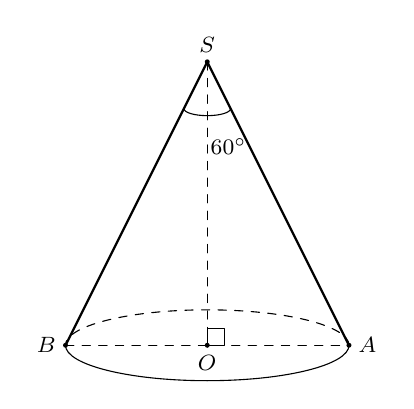
\begin{tikzpicture}[line cap=round,line join=round,>=stealth,x=1.0cm,y=1.0cm,scale=0.9,font=\footnotesize]
		
		\draw[dashed,thin] (5,1) arc (0:180:2 cm and 0.5 cm);
		\draw (1,1) arc (180:360:2 cm and 0.5 cm);
		\draw (2.67,4.34) arc (180:360:0.33 cm and 0.1 cm);
		\draw [line width=0.8pt] (3.,5.)-- (1.,1.);
		\draw [line width=0.8pt] (3.,5.)-- (5.,1.);
		\fill (3,5) circle (1pt) node [above] {$ S $} (1,1) circle (1pt) node [left] {$ B $} (5,1) circle (1pt) node [right] {$ A $} (3,1) circle (1pt) node [below] {$ O $}; 
		\draw (3.3,3.8) node  { \footnotesize $ 60^{\circ}$};
		\draw (3,1) rectangle (3.24,1.24);
		\draw[dashed] (3,5)--(3,1) (1,1)--(5,1);	
	\end{tikzpicture} 
}
	}
\end{ex}

\begin{ex}%[Đề thi thử TN THPT Lần 3, THPT Chuyên Thái Bình năm 2023]%[BCTuan, dự án 12EX6-2023]%[2H2B1-2]%Câu 25
	Cho hình trụ có thiết diện đi qua trục là một hình vuông có cạnh $4a$. Diện tích xung quanh của hình trụ là
	\choice
	{$S=8\pi a^2$}
	{$S=24\pi a^2$}
	{\True $S=16\pi a^2$}
	{$S=4\pi a^2$}
	\loigiai{
	\immini
	{
		Vì thiết diện qua trục là hình vuông có cạnh bằng $4a$ nên chiều cao $h=4a$, bán kính đáy $R=2a$.\\
		Vậy
		$S_{\text{xq}}=2\pi Rh=2\pi\cdot 2a\cdot 4a=16\pi a^2$.
	}
	{
		\begin{tikzpicture}[>=stealth,x=1cm,y=1cm,scale=0.7,line cap=round,line join=round,font=\footnotesize]
			\coordinate (O) at ($(0,0)$);\coordinate (O') at ($(0,4)$);
			\coordinate (A) at ($(-2,0)$);\coordinate (A') at ($(-2,4)$);
			\coordinate (B) at ($(2,0)$);\coordinate (B') at ($(2,4)$);
			\coordinate (S) at ($(0,3.464)$);
			\draw[dashed] (B) arc(0:180: 2 cm and .7 cm);
			\draw (A) arc(180:360: 2 cm and .7 cm);
			\draw (B') arc(0:180: 2 cm and .7 cm);
			\draw (A') arc(180:360: 2 cm and .7 cm);
			\draw[dashed] (A)--(B);\draw[dashed] (O)--(O');
			\draw (A)--(A')--(B')--(B);
		\draw[fill=black] (O) circle (1pt) (O') circle (1pt);
		\end{tikzpicture}
	}
	}
\end{ex}

\begin{ex}%[Đề thi thử TN THPT Lần 3, THPT Chuyên Thái Bình năm 2023]%[BCTuan, dự án 12EX6-2023]%[2D3B1-1]%Câu 26
	Tìm nguyên hàm $F(x)$ của hàm số $f(x)=2x+1-\dfrac{2}{x-2}$ biết $F(1)=3$.
	\choice
	{$F(x)=x^2+x-2\ln (2-x)+1$}
	{$F(x)=x^2+x+2\ln |x-2|+1$}
	{$F(x)=x^2+x-\ln |x-2|+1$}
	{\True $F(x)=x^2+x-2\ln |x-2|+1$}
	\loigiai{
		Ta có
		$F(x)=\displaystyle\int \left(2x+1-\dfrac{2}{x-2}\right)\mathrm{\,d}x=x^2+x-2\ln |x-2|+C$.\\
		Mà $F(1)=3\Rightarrow C=1$.\\ 
		Vậy $F(x)=x^2+x-2\ln |x-2|+1$.}
\end{ex}

\begin{ex}%[Đề thi thử TN THPT Lần 3, THPT Chuyên Thái Bình năm 2023]%[BCTuan, dự án 12EX6-2023]%[2D1Y4-1]%Câu 27
	Đường tiệm cận đứng của đồ thị hàm số $y=\dfrac{x-1}{x-2}$ là 
	\choice
	{$y=1$}
	{$x=1$}
	{\True $x=2$}
	{$y=2$}
	\loigiai{
		Tập xác định $\mathscr{D}=\mathbb{R}\setminus \{2\}$.\\
		Vì $\lim\limits_{x\to 2^+}y=\lim\limits_{x\to 2^+}\dfrac{x-1}{x-2}=+\infty $ nên đường thẳng $x=2$ là tiệm cận đứng của đồ thị hàm số.}
\end{ex}

\begin{ex}%[Đề thi thử TN THPT Lần 3, THPT Chuyên Thái Bình năm 2023]%[BCTuan, dự án 12EX6-2023]%[2D1B3-1]
	Giá trị nhỏ nhất của hàm số $y=x^3-3x+5$ trên đoạn $[2;4]$ là
	\choice
	{$\min\limits_{[2;4]} y=3$}
	{\True $\min\limits_{[2;4]} y=7$}
	{$\min\limits_{[2;4]} y=5$}
	{$\min\limits_{[2;4]} y=0$}
	\loigiai
	{
		Hàm số liên tục trên đoạn $[2;4]$.\\
		Ta có $y'=3x^2-3$. Khi đó
		$y'=0 \Leftrightarrow 3x^2-3=0 \Leftrightarrow \hoac{& x=1 \notin [2;4]\\ & x=-1 \notin [2;4].}$\\
		Lại có $y(2)=7$, $y(4)=57$.\\
		Vậy $\min\limits_{[2;4]} y=7$.
	}
\end{ex}

\begin{ex}%[Đề thi thử TN THPT Lần 3, THPT Chuyên Thái Bình năm 2023]%[BCTuan, dự án 12EX6-2023]%[2D1Y1-2]%Câu 29
	Cho hàm số $y=f(x)$ có bảng biến thiên như sau
	\begin{center}
		
\begin{tikzpicture}
			\tkzTabInit[lgt=1.2,espcl=2.5,deltacl=0.6,nocadre=false]
			{$x$/0.8,$y'$/0.8,$y$/2.5}
			{$-\infty$,$-1$,$0$,$1$,$+\infty$}
			\tkzTabLine{ ,+,0,-,0,+,0,-, }
			\tkzTabVar{-/$-\infty$,+/$2$,-/$1$,+/$2$,-/$-\infty$}
		\end{tikzpicture}
	\end{center}
	Hàm số $y=f(x)$ nghịch biến trên khoảng nào dưới đây?
	\choice
	{$(-\infty ;-1)$}
	{$(0;1)$}
	{\True $(-1;0)$}
	{$(-1;1)$}
	\loigiai{
		Dựa vào bảng biến thiên, hàm số nghịch biến trên các khoảng $(-1;0)$ và $(1;+\infty)$.}
\end{ex}

\begin{ex}%[Đề thi thử TN THPT Lần 3, THPT Chuyên Thái Bình năm 2023]%[BCTuan, dự án 12EX6-2023]%[2D3Y2-1]%Câu 30
	Cho $I=\displaystyle\int\limits_0^2f(x)\mathrm{\,d}x=3$. Khi đó $J=\displaystyle\int\limits_0^2\left[4f(x)-3\right]\mathrm{\,d}x$ bằng 
	\choice
	{$2$}
	{\True $6$}
	{$8$}
	{$4$}
	\loigiai{
		Ta có $J=\displaystyle\int\limits_0^2\left[4f(x)-3\right]\mathrm{\,d}x=4\cdot\displaystyle\int\limits_0^2f(x)\mathrm{\,d}x-\displaystyle\int\limits_0^23\mathrm{\,d}x=4\cdot 3-6=6$.}
\end{ex}

\begin{ex}%[Đề thi thử TN THPT Lần 3, THPT Chuyên Thái Bình năm 2023]%[BCTuan, dự án 12EX6-2023]%[2D3Y2-1]%Câu 31
	Nếu $\displaystyle\int\limits_{-2}^2f(x)\mathrm{\,d}x=9$ và $\displaystyle\int\limits_1^2f(x)\mathrm{\,d}x=2$ thì $\displaystyle\int\limits_{-2}^1f(x)\mathrm{\,d}x$ bằng
	\choice
	{\True $7$}
	{$3$}
	{$11$}
	{$-7$}
	\loigiai{
		Ta có
		$\displaystyle\int\limits_{-2}^2f(x)\mathrm{\,d}x=\displaystyle\int\limits_{-2}^1f(x)\mathrm{\,d}x+\displaystyle\int\limits_1^2f(x)\mathrm{\,d}x
			\Leftrightarrow 9=\displaystyle\int\limits_{-2}^1f(x)\mathrm{\,d}x+2
			\Leftrightarrow\displaystyle\int\limits_{-2}^1f(x)\mathrm{\,d}x=7$.
}
\end{ex}

\begin{ex}%[Đề thi thử TN THPT Lần 3, THPT Chuyên Thái Bình năm 2023]%[BCTuan, dự án 12EX6-2023]%[2D3B2-1]
	Tính $I=\displaystyle\int\limits_0^1\left(\dfrac{1}{2 x+1}+3\sqrt{x}\right)\mathrm{\,d}x$.
	\choice
	{\True $ 2+\ln \sqrt{3}$}
	{$ 4+\ln 3$}
	{$ 2+\ln 3$}
	{$ 1+\ln \sqrt{3}$}
	\loigiai{
		Ta có 
		\allowdisplaybreaks
		\begin{eqnarray*}
			I=\displaystyle\int\limits_{0}^{1}\left(\dfrac{1}{2 x+1}+3 \sqrt{x}\right) \mathrm{d} x&=& \displaystyle\int\limits_{0}^{1} \dfrac{1}{2 x+1} \mathrm{\,d} x+3 \displaystyle\int\limits_{0}^{1} \sqrt{x} \mathrm{\,d} x \\ 
			&=& \dfrac{1}{2} \ln |2 x+1|\bigg|_{0} ^{1}+3 \cdot \dfrac{2}{3} x \sqrt{x}\bigg|_{0} ^{1}\\ 
			&=& \dfrac{1}{2} \ln 3+2=\ln \sqrt{3}+2.
		\end{eqnarray*}
	}
\end{ex}

\begin{ex}%[Đề thi thử TN THPT Lần 3, THPT Chuyên Thái Bình năm 2023]%[BCTuan, dự án 12EX6-2023]%[2H3K2-3]%Câu 33
	Trong KG $Oxyz$, cho $H(1;1;-3)$. Phương trình mặt phẳng $(P)$ đi qua $H$ và cắt các trục tọa độ $Ox$, $Oy$, $Oz$ lần lượt tại $A$, $B$, $C$ sao cho $H$ là trực tâm tam giác $ABC$ là
	\choice
	{$x+y+3z+7=0$}
	{$x+y-3z+11=0$}
	{\True $x+y-3z-11=0$}
	{$x+y+3z-7=0$}
	\loigiai{
\immini
{
Ta có $\heva{&
			AB\perp OC\\&
			AB\perp CH} \Rightarrow AB\perp(OHC)\Rightarrow AB\perp OH$.\\
		Tương tự $\heva{&
			BC\perp OA\\&
			BC\perp OH} \Rightarrow BC\perp(OAH)\Rightarrow BC\perp OH$.\\
		Ta có $\heva{&
			AB\perp OH\\&
			BC\perp OH} \Rightarrow OH\perp(ABC)$.\\
		Do $OH\perp(ABC)$ nên $\overrightarrow{n}_P=\overrightarrow{OH}=(1;1;-3)$.\\
		Phương trình mặt phẳng $(P)$ là
		$$1\cdot(x-1)+1\cdot(y-1)-3\cdot(z+3)=0\Leftrightarrow x+y-3z-11=0.$$
	
}
{
\begin{tikzpicture}[scale=0.8,>=stealth, font=\footnotesize, line join=round, line cap=round]
	\path
	(0,0) coordinate (O) 
	(90:3) coordinate (C)
	(90:4) coordinate (z)
	(10:5) coordinate (B)
	(10:6) coordinate (y)
	(-20:3) coordinate (A)
	(-20:4) coordinate (x)
	(40:2) coordinate (H)
	;
	\draw 
	(O)--(A)--(B)--(C)--cycle
	(A)--(C)
	;
	\draw[dashed] (O)--(B) (O)--(H);
	\draw[->] (C)--(z); \draw[->](B)--(y);\draw[->] (A)--(x);
	\foreach \x/\g in
	{A/-90,B/90,C/180,O/-90,H/0}
	\fill[black](\x) circle (2pt)
	($(\x)+(\g:5mm)$) node{$\x$};
	\foreach \x/\g in
	{x/-90,y/-90,z/90}
	\fill[black](\x) circle (0pt)
	($(\x)+(\g:5mm)$) node{$\x$};
\end{tikzpicture}
}
}
\end{ex}

\begin{ex}%[Đề thi thử TN THPT Lần 3, THPT Chuyên Thái Bình năm 2023]%[BCTuan, dự án 12EX6-2023]%[2H3K2-3]%Câu 34
	Trong KG $Oxyz$, mặt phẳng $(P)$ đi qua điểm $A(1;1;3)$ và chứa trục hoành có phương trình là
	\choice
	{$3y+z-4=0$}
	{\True $3y-z=0$}
	{$x-y=0$}
	{$x-3y=0$}
	\loigiai{
		Ta có $\overrightarrow{OA}=(1;1;3)$, $\overrightarrow{i}=(1;0;0)$.\\
		Mặt phẳng $(P)$ qua $A$ và chứa $Ox$ nên $(P)$ có véc-tơ pháp tuyến $\overrightarrow{n}_P=\left[\overrightarrow{OA},\overrightarrow{i}\right]=(0;3;-1)$.\\
		Suy ra $(P)\colon 0\cdot (x-1)+3\cdot (y-1)-1\cdot (z-3)=0\Leftrightarrow 3y-z=0$.
	}
\end{ex}

\begin{ex}%[Đề thi thử TN THPT Lần 3, THPT Chuyên Thái Bình năm 2023]%[BCTuan, dự án 12EX6-2023]%[2D2K5-5]%Câu 35
	Cho hàm số $y=f(x)$ liên tục trên $\mathbb{R}$ và có đồ thị như hình vẽ dưới đây. Có bao nhiêu giá trị nguyên của tham số $m$ để phương trình $f(3\log_3x)=m-1$ có nghiệm duy nhất trên $\left[\dfrac{1}{\sqrt[3]{3}};3\right)$?
	\begin{center}
		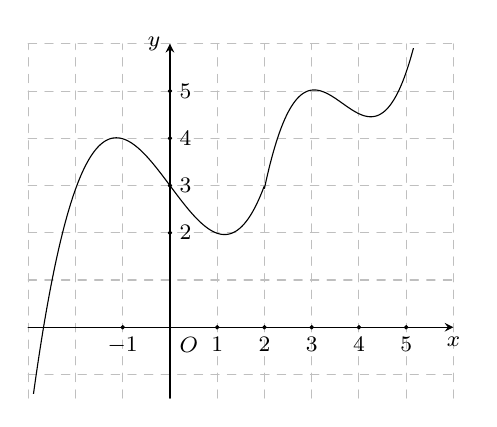
\begin{tikzpicture}[scale=0.6,>=stealth, font=\footnotesize, line join=round, line cap=round]
			\def\xmin{-3} \def\xmax{6}
			\def\ymin{-1.5} \def\ymax{6} 
			\draw[color=gray!50,dashed] (\xmin,\ymin) grid (\xmax,\ymax); 
			\draw[->] (\xmin,0)--(\xmax,0) node [below]{$x$};
			\draw[->] (0,\ymin)--(0,\ymax) node [left]{$y$};
			\node at (0,0) [below right]{$O$};
			\clip (\xmin+0.1,\ymin+0.1) rectangle (\xmax-0.5,\ymax-0.1);
			\draw[smooth,samples=300,domain=\xmin:2] plot(\x,{0.34*(\x)^3-0.01*(\x)^2-1.34*(\x)+3});
			\draw[smooth,samples=300,domain=2:\xmax] plot(\x,{0.66*(\x)^3-7.23*(\x)^2+25.69*(\x)-24.8});
			\draw[fill=black]
			(0,2)node[right]{$2$}circle(1pt)
			(0,3)node[right]{$3$}circle(1pt)
			(0,4)node[right]{$4$}circle(1pt)
			(0,5)node[right]{$5$}circle(1pt)
			(-1,0)node[below]{$-1$}circle(1pt)
			(1,0)node[below]{$1$}circle(1pt)
			(2,0)node[below]{$2$}circle(1pt)
			(3,0)node[below]{$3$}circle(1pt)
			(4,0)node[below]{$4$}circle(1pt)
			(5,0)node[below]{$5$}circle(1pt)
			;
		\end{tikzpicture}
	\end{center}
	\choice
	{$2$}
	{$4$}
	{$3$}
	{\True $1$}
	\loigiai{
		Điều kiện $\dfrac{1}{\sqrt[3]{3}}\le x < 3$.\\
		Đặt $t=3\log_3x$, vì $\dfrac{1}{\sqrt[3]{3}}\le x < 3\Rightarrow -1\le t<3$, phương trình đã cho trở thành phương trình
		$f(t)=m-1.\quad (1)$\\
		Ta cần tìm $m$ để phương trình $(1)$ có nghiệm duy nhất $t\in[-1;3)$.\\
		Dựa vào đồ thị đã cho, ta thấy yêu cầu bài toán được thỏa mãn khi và chỉ khi $\heva{&
			m-1=2\\&
			4<m-1<5} \Leftrightarrow \heva{&
			m=3\\&
			5<m<6.}$\\
		Mà $m$ là số nguyên nên $m=3$.}
\end{ex}

\begin{ex}%[Đề thi thử TN THPT Lần 3, THPT Chuyên Thái Bình năm 2023]%[BCTuan, dự án 12EX6-2023]%[2D3B2-1]%Câu 36
	Cho hàm số $f(x)$ liên tục và có đạo hàm trên $[1;3]$, $f(3)=4$ và $\displaystyle\int\limits_0^1f'(2x+1)\mathrm{\,d}x=6$. Tính giá trị của $f(1)$.
	\choice
	{\True $f(1)=-8$}
	{$f(1)=-2$}
	{$f(1)=16$}
	{$f(1)=10$}
	\loigiai{
		Ta có $\displaystyle\int\limits_0^1f'(2x+1)\mathrm{\,d}x=6$.\\
		Đặt $t=2x+1\Rightarrow \mathrm{d}t=2\mathrm{\,d}x$.\\
Đổi cận:
			$x=0\Rightarrow t=1, 
			x=2\Rightarrow t=3$.\\
			Suy ra $6=\dfrac{1}{2}\displaystyle\int\limits_1^3f'(t)\mathrm{\,d}t=\dfrac{1}{2}f(t)\bigg|_0^3=\dfrac{1}{2}\left[f(3)-f(1)\right]=\dfrac{1}{2}\left[4-f(1)\right]$.\\
			Suy ra $f(1)=-8$.
	}
\end{ex}

\begin{ex}%[Đề thi thử TN THPT Lần 3, THPT Chuyên Thái Bình năm 2023]%[BCTuan, dự án 12EX6-2023]%[1H3B5-4]%Câu 37
	Cho hình chóp $S.ABCD$ có đáy là hình vuông cạnh $a$, đường thẳng $SA$ vuông góc với mặt phẳng $(ABCD)$, $SA=a\sqrt{2}$. Khoảng cách giữa hai đường thẳng $SB$ và $AD$ bằng
	\choice
	{\True $\dfrac{a\sqrt{6}}{3}$}
	{$\dfrac{a\sqrt{2}}{3}$}
	{$\dfrac{a\sqrt{3}}{2}$}
	{$a$}
	\loigiai{
	\immini
	{
		Gọi $H$ là hình chiếu của $A$ lên $SB$. Ta có $AH\perp SB$.\\
		Do tứ giác $ABCD$ là hình vuông nên $AD\perp AB$.\\
		Do $SA$ vuông góc với mặt phẳng $(ABCD)$ nên $AD\perp SA$\\
		Suy ra $ AD\perp(SAB)\Rightarrow AD\perp AH$.\\
		Từ đó suy ra $AH$ là đoạn vuông góc chung của $AD$ và $SB$ nên $\mathrm{d}(SB,AD)=AH$.\\
		Xét tam giác $SAB$ vuông tại $A$ đường cao $AH$ ta có\\
		$$\dfrac{1}{AH^2}=\dfrac{1}{SA^2}+\dfrac{1}{AB^2}=\dfrac{1}{2a^2}+\dfrac{1}{a^2}=\dfrac{3}{2a^2}\Leftrightarrow AH=\dfrac{a\sqrt{6}}{3}.$$ 
		Vậy $\mathrm{d}(SB,AD)=\dfrac{a\sqrt{6}}{3}$.
	}
	{
	\begin{tikzpicture}[scale=0.7, font=\footnotesize, line join=round, line cap=round, >=stealth]
		\def\bc{4} % cạnh BC
		\def\ba{2} % cạnh BA
		\def\h{3} % đường cao
		\def\gocB{30} % góc B của đáy
		\coordinate[label=below left:$B$] (B) at (0,0);
		\coordinate[label=below:$A$] (A) at (\gocB:\ba);
		\coordinate[label=below:$C$] (C) at (\bc,0);
		\coordinate[label=right:$D$] (D) at ($(C)-(B)+(A)$);
		\coordinate[label=above:$S$] (S) at ($(A)+(90:\h)$);
		\coordinate[label=above left:$H$] (H) at ($(S)!0.5!(B)$);
		\draw (B)--(C)--(D)--(S)--cycle (S)--(C);
		\draw[dashed] (H)--(A)--(D) (S)--(A)--(B);
		\foreach \diem in {A,B,C,D,S,H}	\fill (\diem)circle(1pt);
	\draw pic[draw,angle radius=2mm] {right angle = D--A--S};
	\end{tikzpicture}
	}
	}
\end{ex}

\begin{ex}%[Đề thi thử TN THPT Lần 3, THPT Chuyên Thái Bình năm 2023]%[BCTuan, dự án 12EX6-2023]%[2H3B1-3]%Câu 38
	Trong KG $Oxyz$, cho $A(1;2;3)$, $B(4;2;3)$, $C(4;5;3)$. Diện tích mặt cầu nhận đường tròn ngoại tiếp tam giác $ABC$ làm đường tròn lớn là
	\choice
	{$9\pi $}
	{$36\pi $}
	{\True $18\pi $}
	{$72\pi $}
\loigiai{
	Ta có $AB=3, AC=3\sqrt{2}, BC=3$.\\ 
	Do đó tam giác $ABC$ vuông cân tại $B$ và bán kính đường tròn ngoại tiếp tam giác $ABC$ là $R=\dfrac{1}{2}AC=\dfrac{3\sqrt{2}}{2}$.\\
	Mặt cầu nhận đường tròn ngoại tiếp tam giác $ABC$ làm đường tròn lớn, suy ra bán kính đường tròn ngoại tiếp tam giác $ABC$ là bán kính mặt cầu.\\
	Diện tích mặt cầu $S=4\pi\cdot R^2 =18\pi$.
}
\end{ex}

%D:\Nguyen Tuan\THU MUC DOWNLOAD\HINH OXY 2016\12EX-6-2023\2-TT\2-TT-10-ChuyenThaiBinh-23-L3.tex
\begin{ex}%[Đề thi thử TN THPT Lần 3, THPT Chuyên Thái Bình năm 2023]%[BCTuan, dự án 12EX6-2023]%[2D1B1-1]%Câu 39
	Cho hàm số $y=f(x)$ có xác định trên và có đạo hàm $f'(x)=(x-1)^2x(x+1)$. Hàm số đã cho nghịch biến trên khoảng nào dưới đây?
	\choice
	{\True $(-1;0)$}
	{$(-\infty ;-1)$}
	{$(0;1)$}
	{$(1;+\infty)$}
	\loigiai{
		Ta có $f'(x)=(x-1)^2x(x+1)=0\Leftrightarrow\hoac{&
			x=1\\&
			x=0\\&
			x=-1}$, với $x=1$ là nghiệm bội chẵn.\\
		Bảng xét dấu đạo hàm $f'(x)$
\begin{center}
	
\begin{tikzpicture}
		\tkzTabInit[lgt=1.3,espcl=3,deltacl=0.6,nocadre=false]
		{$x$/1,$f'(x)$/1}
		{$-\infty$,$-1$,$0$,$1$,$+\infty$}
		\tkzTabLine{ ,+,0,-,0,+,0,+, }
	\end{tikzpicture}
\end{center}
		Căn cứ vào bảng xét dấu thì hàm số nghịch biến trên khoảng $(-1;0)$.}
\end{ex}

\begin{ex}%[Đề thi thử TN THPT Lần 3, THPT Chuyên Thái Bình năm 2023]%[BCTuan, dự án 12EX6-2023]%[2H3B2-7]%Câu 40
	Trong KG $Oxyz$, mặt cầu $(S)$ có tâm $I(1;-2;-1)$ và có tiếp diện là mặt phẳng $(P)\colon 2x+y+2z+5=0$, có phương trình là
	\choice
	{$(x-1)^2+(y+2)^2+(z+1)^2=4$}
	{$(x+1)^2+(y-2)^2+(z-1)^2=1$}
	{$(x+1)^2+(y-2)^2+(z-1)^2=4$}
	{\True $(x-1)^2+(y+2)^2+(z+1)^2=1$}
	\loigiai{
		Bán kính của mặt cầu $(S)$ là $R=\mathrm{d}(I,(P))=\dfrac{\left|2\cdot 1-1\cdot 2-2\cdot 1+5\right|}{\sqrt{2^2+1^2+2^2}}=1$.\\
		Phương trình mặt cầu $(S)$ là $(x-1)^2+(y+2)^2+(z+1)^2=1$.}
\end{ex}

\begin{ex}%[Đề thi thử TN THPT Lần 3, THPT Chuyên Thái Bình năm 2023]%[BCTuan, dự án 12EX6-2023]%[2D3K2-4]%Câu 41
	Cho $f(x)$ là một hàm số liên tục trên tập số thực không âm và $f(x^2+3x+1)=x+2$, $\forall x\ge 0$. Tính $\displaystyle\int\limits_1^5f(x)\mathrm{\,d}x$.
	\choice
	{$\dfrac{37}{6}$}
	{$\dfrac{527}{3}$}
	{\True $\dfrac{61}{6}$}
	{$\dfrac{464}{3}$}
	\loigiai{
	Ta có 
	\begin{eqnarray*}
		f(x^2+3x+1)=x+2&\Leftrightarrow&(2x+3)f(x^2+3x+1)=(2x+3)(x+2)\\
		& \Leftrightarrow & (2x+3)f(x^2+3x+1)=2x^2+7x+6.
	\end{eqnarray*}
	Khi đó,
	\begin{eqnarray*}
		&&\displaystyle\int\limits_0^1(2x+3)f(x^2+3x+1)\mathrm{\,d}x=\displaystyle\int\limits_0^1(2x^2+7x+6)\mathrm{\,d}x\\
		& \Leftrightarrow & \displaystyle\int\limits_0^1(2x+3)f(x^2+3x+1)\mathrm{\,d}x=\left(\dfrac{2}{3}x^3+\dfrac{7x^2}{2}+6x\right)\bigg|_0^1=\dfrac{61}{6}.
	\end{eqnarray*}
Xét tích phân $\displaystyle\int\limits_0^1(2x+3)f(x^2+3x+1)\mathrm{\,d}x$.\\
Đặt $t=x^2+3x+1\Rightarrow \mathrm{\,d}t=(2x+3)\mathrm{\,d}x$.\\
Đổi cận: $x=0\Rightarrow t=1$, $x=1\Rightarrow t=5$.\\
Vậy $\displaystyle\int\limits_0^1(2x+3)f(x^2+3x+1)\mathrm{\,d}x=\displaystyle\int\limits_1^5 f(t) \mathrm{\,d}t=\dfrac{61}{6}$.\\
	Vậy $\displaystyle\int\limits_1^5f(x)\mathrm{\,d}x=\dfrac{61}{6}$.	
	}
\end{ex}

\begin{ex}%[Đề thi thử TN THPT Lần 3, THPT Chuyên Thái Bình năm 2023]%[BCTuan, dự án 12EX6-2023]%[1H3B3-3]%Câu 42
	Cho hình lăng trụ đứng $ABC.A'B'C'$ có đáy $ABC$ vuông tại $A$, $AB=a\sqrt{3}$, $AC=AA'=a$. Giá trị sin của góc giữa đường thẳng $AC'$ và mặt phẳng $(BCC'B')$ bằng 
	\choice
	{$\dfrac{\sqrt{10}}{4}$}
	{$\dfrac{\sqrt{6}}{3}$}
	{$\dfrac{\sqrt{3}}{3}$}
	{\True $\dfrac{\sqrt{6}}{4}$}
	\loigiai{
		\immini{
			Kẻ $AH\perp BC$ tại $H$. Ta có $\heva{& AH \perp BC \\ & AH \perp BB'}\Rightarrow AH \perp (BCC'B')$.\\
			Vậy $C'H$ là hình chiếu vuông góc của $AC'$ lên $(BCC'B')$. Góc giữa $AC'$ và $(BCC'B')$ là $\widehat{AC'H}$. Ta có
			\begin{itemize}
				\item $AC'=\sqrt{CC'^2+AC^2}=a\sqrt{2}$;
				\item $AH=\dfrac{AB\cdot AC}{\sqrt{AB^2+AC^2}}=\dfrac{\sqrt{3}a}{2}$;
				\item $\sin \widehat{AC'H}=\dfrac{AH}{AC'}=\dfrac{\sqrt{6}}{4}$.
			\end{itemize}
			
		}{
			\begin{tikzpicture}[scale=0.8, font=\footnotesize, line join=round, line cap=round, >=stealth]
				\path
				(0,0) coordinate (A)
				(2,-1.5) coordinate (B)
				(3.5,0) coordinate (C)
				($(B)!0.6!(C)$) coordinate (H)
				(0,-4) coordinate (A')
				($(A')+(B)-(A)$) coordinate (B')
				($(B')+(C)-(B)$) coordinate (C')
				;
				\draw 
				(A)--(B)--(C)--cycle
				(A')--(B')--(C')
				(A)--(H)--(C')
				(A)--(A') (B)--(B') (C)--(C')
				;
				\draw[dashed] 
				(A)--(C')--(A')
				;
				\foreach \p/\g in {A/180/, B/90, C/30, H/-30, A'/180, B'/-90, C'/-30}
				\draw[fill=black] (\p) circle (1pt) node[shift=(\g:3mm)] {$\p$};
				\pic[draw,angle radius=2mm]{right angle = A--H--B};
				\pic[draw,angle radius=2mm]{right angle = B'--A'--C'};
			\end{tikzpicture}
		}
	}
\end{ex}

\begin{ex}%[Đề thi thử TN THPT Lần 3, THPT Chuyên Thái Bình năm 2023]%[BCTuan, dự án 12EX6-2023]%[2D1G3-1]%Câu 43
	Cho hàm số $f(x)=x^2-2x+1$. Gọi $S$ là tập hợp tất cả các giá trị thực của tham số $m$ để giá trị lớn nhất của hàm số $g(x)=\left|f^2(x)-2f(x)+m\right|$ trên đoạn $[-1;3]$ bằng $8$. Tính tổng các phần tử của $S$.
	\choice
	{\True $-7$}
	{$2$}
	{$0$}
	{$5$}
	\loigiai{
	Xét hàm số $f(x)$, ta có bảng biến thiên
	\begin{center}
		\begin{tikzpicture}[scale=0.7,line join=round, line cap=round,>=stealth]
			\tkzTabInit[nocadre=false,lgt=2,espcl=2,deltacl=1]
			{$x$/1,$f(x)$/2}
			{$-1$,$1$,$2$,$3$}
			\draw 
			(N11)node[below](A){$4$}
			(N22)node[above](B){$0$}
			(N41)node[below](E){$4$}
			($(B)!1/2!(E)$)node (C){$1$}
			;
			\draw[->] (A)--(B);
			\draw[->] (B)--(C) (C)--(E);
		\end{tikzpicture}
	\end{center}
	Đặt $u=f(x)$, từ bảng biến thiên ta thấy $u \in [0;4]$. Suy ra $g(u)=|f(u)+m-1|, u\in [0;4]$.\\
	Bảng biến thiên của $f(u)$ trên đoạn $[0;4]$ như sau:
	\begin{center}
		\begin{tikzpicture}[scale=1,line join=round, line cap=round,>=stealth]
			\tkzTabInit[nocadre=false,lgt=1,espcl=2,deltacl=1]
			{$u$/1,$f(u)$/2}
			{$0$,$1$,$4$}
			\draw 
			(N11)node[below](A){$1$}
			(N22)node[above](B){$0$}
			(N31)node[below](E){$9$}
			;
			\draw[->] (A)--(B);
			\draw[->] (B)--(E);
		\end{tikzpicture}
	\end{center}
	Suy ra trên đoạn $[0;4]$ thì $0\le f(u)\le 9$, do đó
	$$\max\limits_{[0;4]} g(u)=\max \{|m-1|,|m+8|\}. $$
	{\bf TH1.} $\max\limits_{[0;4]} g(u)=|m-1|$. Suy ra
	$$\heva{&|m-1|=8\\&|m-1|\ge |m+8|\\}\Rightarrow \heva{&\hoac{&m=9\\&m=-7\\}\\&|m-1|\ge |m+8|}\Rightarrow m=-7.$$
	{\bf TH2.} $\max\limits_{[0;4]} g(u)=|m+8|$. Suy ra
	$$\heva{&|m+8|=8\\&|m-1|\le |m+3|}\Rightarrow \heva{&\hoac{&m=0\\&m=-16\\}\\&|m-1|\le |m+3|\\}\Rightarrow m=0.$$
	Vậy có hai giá trị của $m$ thỏa mãn là $m=0$ hoặc $m=-7$.\\ 	
	 Tổng các giá trị của $m$ thỏa mãn bằng $7$.
	}
\end{ex}
\begin{ex}%[Đề thi thử TN THPT Lần 3, THPT Chuyên Thái Bình năm 2023]%[BCTuan, dự án 12EX6-2023]%[2D1G2-2]
	\immini
	{Cho hàm số $y=f(x)$ liên tục trên $\mathbb{R}$. Đồ thị hàm số $f'(\sqrt[3]{x})$ được cho trong hình bên. Hàm số $g( x )=\left| f(x)-\dfrac{1}{8}x^4-x \right|$ có tối đa bao nhiêu điểm cực đại?
		\choice
		{$2$}
		{$4$}
		{$5$}
		{\True $3$}
	}
	{	
		\begin{tikzpicture}[scale=0.9, font=\footnotesize, line join=round, line cap=round, >=stealth]
			\draw[->] (-3,0)--(3.5,0)node[below]{$x$};
			\draw[->] (0,-2)--(0,4)node[right]{$y$};
			\draw[samples=150,smooth,domain=-2.2:2.2] plot(\x,{5/6*(\x)^3-17/6*(\x)+1});
			\node [below left] at (0,0) {$ O $};
			\node [above left] at (-2,0) {$ -2 $};
			\node [left] at (0,1) {$ 1 $};
			\draw[dashed] (2,0) node [below ] {$ 2 $}--(2,2)--(0,2) node [left] {$ 2 $};
		\end{tikzpicture}	
	}
	\loigiai{
		Xét hàm số $h(x)=f(x)-\dfrac{1}{8}x^4-x$ liên tục trên $\mathbb{R}$.\\
		Ta có $h'(x)=f'(x)-\dfrac{1}{2}x^3-1$, $h'( x )=0\Leftrightarrow f'(x)=\dfrac{1}{2}x^3+1$.\\
		Đặt $x=\sqrt[3]{t}\Rightarrow t=x^3$, xét phương trình $f'(\sqrt[3]{t})-\left(\dfrac{1}{2}t+1 \right)=0$.\\
		Vẽ đồ thị hàm số $y=\dfrac{1}{2}t+1$ và đồ thị hàm số $y=f'(\sqrt[3]{t})$ trên cùng hệ trục tọa độ $ Oty $ như hình vẽ
		\begin{center}
			\begin{tikzpicture}[scale=1, font=\footnotesize, line join=round, line cap=round, >=stealth]
				\draw[->] (-3,0)--(4.5,0)node[below]{$t$};
				\draw[->] (0,-2)--(0,4)node[right]{$y$};
				\draw[samples=150,smooth,domain=-2.2:2.2] plot(\x,{5/6*(\x)^3-17/6*(\x)+1});
				\draw[thick,samples=150,smooth,domain=-2.5:2.5] plot(\x,{1/2*(\x)+1});
				\node [below left] at (0,0) {$ O $};
				\node [above left] at (-2,0) {$ -2 $};
				\node [above left] at (0,1) {$ 1 $};
				\draw[dashed] (2,0) node [below ] {$ 2 $}--(2,2)--(0,2) node [above left] {$ 2 $};
				\node [above] at (2,3.5) {$ y=f'( \sqrt[3]{t} ) $};
				\node [above] at (3.5,2.2) {$ y=\dfrac{1}{2}t+1 $};
			\end{tikzpicture}
		\end{center}
		Dựa vào đồ thị trên ta có $h'( x)=0\Rightarrow f'(\sqrt[3]{t})-\left(\dfrac{1}{2}t+1\right )=0 \Rightarrow  \hoac{&t=-2 \\&t=0 \\&t=2}\Rightarrow \hoac{&x=-\sqrt[3]{2}\\&x=0 \\&x=\sqrt[3]{2}.}$\\
		Ta có bảng biến thiên của hàm số $h(x)$ như sau
		\begin{center}
			% Cần khai báo \usepackage{tkz-tab}
			
\begin{tikzpicture}[>=stealth]
				\tkzTabInit[nocadre=false,lgt=1.2,espcl=2.5,deltacl=0.6]{$x$ /0.6,$h’(x)$ /0.6,$h(x)$ /2}
				{$-\infty$ , $-\sqrt[3]{2}$, $ 0 $ , $ \sqrt[3]{2} $ , $+\infty$}
				\tkzTabLine{ , - , $0$ , + , $0$ , - , $ 0 $, +, }
				\tkzTabVar{+/$+\infty$ , -/$h(-\sqrt[3]{2})$ , +/$h(0)$ , -/$h(\sqrt[3]{2})$, +/$ +\infty $}
			\end{tikzpicture}
			
		\end{center}
		Dựa vào bảng biến thiên của hàm $ h(x) $ suy ra hàm số $g(x)=|h(x)|$ có tối đa $3$ điểm cực đại.
	}
\end{ex}
\begin{ex}%[Đề thi thử TN THPT Lần 3, THPT Chuyên Thái Bình năm 2023]%[BCTuan, dự án 12EX6-2023]%[2H1K3-3]
	Cho hình chóp $S.ABCD$ có đáy $ABCD$ là hình bình hành. Gọi $M$ là điểm đối xứng của $C$ qua $B$ và $N$ là trung điểm của $SC$. Mặt phẳng $(MND)$ chia khối chóp $S.ABCD$ thành hai khối đa diện, trong đó khối đa diện chứa đỉnh $S$ có thể tích $V_1$, khối đa diện còn lại có thể tích $V_2$. Tính tỷ số $\dfrac{V_1}{V_2}$.\\
	\choice
	{ $\dfrac{V_1}{V_2}=\dfrac{12}{7}$}
	{ $\dfrac{V_1}{V_2}=\dfrac{5}{3}$}
	{\True $\dfrac{V_1}{V_2}=\dfrac{7}{5}$}
	{ $\dfrac{V_1}{V_2}=\dfrac{1}{5}$}
	
	\loigiai{
		\immini{Trong tam giác $SMC$, $SB$ và $MN$ là hai trung tuyến cắt nhau tại trọng tâm $K\Rightarrow \dfrac{SK}{SB}=\dfrac{2}{3}$.\\
			Mà $BI$ là đường trung bình của tam giác $MCD\Rightarrow I$ là trung điểm $AB$.\\
			Ta có $V_1={V_{S.AID}}+{V_{S.IKN}}+{V_{S.IND}}$.\\ 
			Gọi ${V_{S.ABCD}}=V$.\\
			Suy ra $\heva{&V_{S.AID}=\dfrac{1}{4}\cdot V\\&{V_{S.IKN}}=\dfrac{SK}{SB}\cdot\dfrac{SN}{SC}\cdot V_{S.IBC}=\dfrac{2}{3}\cdot\dfrac{1}{2}\cdot\dfrac{1}{4}V=\dfrac{1}{12}V\\&{V_{S.IND}}=\dfrac{SN}{SC}\cdot{V_{S.ICD}}=\dfrac{1}{2}\cdot\dfrac{1}{2}V=\dfrac{1}{4}V.}$\\
			Do đó ${V_1}=\left(\dfrac{1}{4}+\dfrac{1}{12}+\dfrac{1}{4}\right)\cdot V=\dfrac{7}{12}\cdot V\Rightarrow {V_2}=\dfrac{5}{12}V$.\\
			Vậy tỉ số $\dfrac{V_1}{V_2}=\dfrac{7}{5}$.}
		{\begin{tikzpicture}[scale=.6, font=\footnotesize, line join=round, line cap=round, >=stealth]
				\def\bc{4.5} % cạnh BC
				\def\ba{3} % cạnh BA
				\def\h{4} % đường cao
				\def\gocB{30} % góc B của đáy
				\path
				(0,0) coordinate (B)
				(\gocB:\ba) coordinate (A)
				(\bc,0)coordinate (C)
				($(C)-(B)+(A)$)coordinate (D)
				($(A)+(90:\h)$)coordinate (S)
				($(A)!.5!(B)$) coordinate (I)
				($(C)!.5!(S)$) coordinate (N)
				(-\bc,0)coordinate (M)
				(intersection of S--B and M--N)coordinate (K)
				;
				\draw (B)--(C)--(D)--(S)--cycle (S)--(C) (D)--(N)--(M) (M)--(B);
				\draw[dashed] (S)--(A)--(D)--(M) (A)--(B) (C)--(I)--(N) (I)--(K);
				\foreach \x/\g in {A/-90, B/-90, C/-40, D/0, M/-90, K/135, S/90, N/45, I/-80} \draw[fill=black] (\x) circle (.03)+(\g:.3) node{$\x$};
		\end{tikzpicture}}
	}
\end{ex}
\begin{ex}%[Đề thi thử TN THPT Lần 3, THPT Chuyên Thái Bình năm 2023]%[BCTuan, dự án 12EX6-2023]%[2D2K4-4]%Câu 46
	Cho hàm số $f(x)=ax-(a-3)\ln (x^2+3x)$ với $a$ là tham số thực. Biết rằng nếu $\max\limits_{[1;3]}f(x)=f(2)$ thì $\min\limits_{[1;3]}f(x)=m$. Khẳng định nào sau đây đúng?
	\choice
	{\True $m\in(6;7)$}
	{$m\in(7;8)$}
	{$m\in(8;9)$}
	{$m\in(9;10)$}
	\loigiai{
		Trên $[1;3]$ hàm số $y=f(x)$ luôn xác định.\\
		Ta có $f'(x)=a-(a-3)\cdot \dfrac{2x+3}{x^2+3x}$.\\
		Vì $\max\limits_{[1;3]}f(x)=f(2)$ nên $f'(2)=0\Rightarrow a-(a-3)\cdot \dfrac{7}{10}=0\Leftrightarrow a=-7$.\\
		Khi đó $f'(x)=-7+\dfrac{20x+30}{x^2+3x}=0\Leftrightarrow \hoac{&
			x=2\\&
			x=-\dfrac{15}{7}.}$\\
		Ta có $f(1)=-7+10\ln 4$, $f(2)=-14+10\ln 10$; $f(3)=-21+10\ln 18$.\\
		Vậy $m=\min\limits_{[1;3]}f(x)=f(1)\approx 6{,}86.$}
\end{ex}

\begin{ex}%[Đề thi thử TN THPT Lần 3, THPT Chuyên Thái Bình năm 2023]%[BCTuan, dự án 12EX6-2023]%[2D3K1-1]%Câu 47
	Cho hàm số $f(x)$ có đạo hàm trên đoạn $[1;\mathrm{e}]$ và thỏa mãn $f(1)=0$, $\left[f'(x)-1\right]x=f(x),\ \forall x\in[1 ;\mathrm{e}]$. Tích phân $\displaystyle\int\limits_1^\mathrm{e}f(x)\mathrm{\,d}x$ bằng
	\choice
	{$\dfrac{\mathrm{e}^2-1}{4}$}
	{$\dfrac{\mathrm{e}^2+1}{2}$}
	{\True $\dfrac{\mathrm{e}^2+1}{4}$}
	{$\dfrac{\mathrm{e}^2-1}{2}$}
	\loigiai{
		Ta có 
		\begin{eqnarray*}
		&&\left[f'(x)-1\right]x=f(x),\ \forall x\in[1 ;\mathrm{e}]\\
		&\Leftrightarrow & xf'(x)-f(x)=x,\ \forall x\in [1;\mathrm{e}]\\
		&\Leftrightarrow &\dfrac{xf'(x)-f(x)}{x^2}=\dfrac{1}{x},\ \forall x\in [1;\mathrm{e}]\\
		&\Leftrightarrow &\left(\dfrac{f(x)}{x}\right)'=\dfrac{1}{x},\ \forall x\in[1;\mathrm{e}].	
		\end{eqnarray*}
		Lấy nguyên hàm hai vế của ta được $\dfrac{f(x)}{x}=\ln x+C\Leftrightarrow f(x)=x\ln x+Cx,\ \forall x\in[1;\mathrm{e}]$.\\
		Mà $f(1)=0\Rightarrow C=0$ .\\
		Vậy $f(x)=x\ln x,\ \forall x\in[1;\mathrm{e}].$\\
		Xét $I=\displaystyle\int\limits_1^\mathrm{e} x\ln x\mathrm{\,d}x$. \\
		Đặt $\heva{&u=\ln x\\&\mathrm{\,d}v=x\mathrm{\,d}x}\Rightarrow\heva{&\mathrm{\,d}u=\dfrac{1}{x}\mathrm{\,d}x\\&v=\dfrac{x^2}{2}.}$ \\
		Khi đó
		\begin{eqnarray*}
			\allowdisplaybreaks
			I&=&\dfrac{x^2}{2}\ln x\bigg|_0^\mathrm{e}-\displaystyle\int\limits_0^\mathrm{e}\dfrac{1}{x}\cdot\dfrac{x^2}{2}\mathrm{\,d}x\\
			&=&\dfrac{\mathrm{e}^2}{2}-\dfrac{1}{2}\displaystyle\int\limits_0^\mathrm{e} x\mathrm{\,d}x\\
			&=&\dfrac{\mathrm{e}^2}{2}-\dfrac{x^2}{4}\bigg|_0^\mathrm{e}\\
			&=&\dfrac{\mathrm{e}^2}{2}-\dfrac{\mathrm{e}^2}{4}+\dfrac{1}{4}\\
			&=&\dfrac{\mathrm{e}^2+1}{4}.
	\end{eqnarray*}
}
\end{ex}

\begin{ex}%[Đề thi thử TN THPT Lần 3, THPT Chuyên Thái Bình năm 2023]%[BCTuan, dự án 12EX6-2023]%[2D2G5-5]%Câu 48
	Có bao nhiêu số nguyên dương $x$ sao cho tồn tại số thực $y$ lớn hơn 1 thỏa mãn $(x{y^2}+x-2y-1)\log y=\log\dfrac{2y-x+3}{x}$?
	\choice
	{$3$}
	{$1$}
	{vô số}
	{\True $2$}
	\loigiai{
		Điều kiện: $\heva{&y>1\\&x\in \mathbb{N}^*\\&\dfrac{2y-x+3}{x}>0.}$\\
		Ta có 
		\begin{eqnarray*}
			&& (xy^2+x-2y-1)\log y=\log \dfrac{2y-x+3}{x}\\
			&\Leftrightarrow & (xy^2+x-2y-3)\log y +2\log y=\log (2y-x+3)-\log x\\
			&\Leftrightarrow & (xy^2+x-2y-3)\log y =\log (2y-x+3)-\log (xy^2).\quad (1)\\
		\end{eqnarray*}
		\begin{itemize}
			\item[•] Nếu $xy^2>2y-x+3$ thì $\heva{&\text{Vế trái}\ >0\\&\text{Vế phải}\ <0}\ \ (\text{do}\ \ \log y>0)$.
			\item[•] Nếu $xy^2<2y-x+3$ thì $\heva{&\text{Vế trái}\ <0\\&\text{Vế phải}\ >0}\ \ (\text{do}\ \ \log y>0)$.
		\end{itemize}
		Do đó, từ $(1)$ suy ra 
		$$xy^2=2y-x+3\Leftrightarrow x=\dfrac{2y+3}{y^2+1}.$$
		Xét hàm số $f(y)=\dfrac{2y+3}{y^2+1}$, $y\in (1;+\infty )$. Ta có 
		$$f'(y)=\dfrac{-2y^2-6y+2}{(y^2+1)^2}<0,\ \ \forall y\in (1;+\infty ).$$
		Suy ra hàm số $f(y)$ nghịch biến trên khoảng $(1;+\infty)$.\\
		Suy ra $x=f(y)\in \left(0;\dfrac{5}{2}\right)$. Vì $x\in \mathbb{N}^*$ nên $x\in \{1;2\}$.\\
		Vậy có hai giá trị nguyên dương $x$ thỏa mãn bài toán.
	}
\end{ex}

\begin{ex}%[Đề thi thử TN THPT Lần 3, THPT Chuyên Thái Bình năm 2023]%[BCTuan, dự án 12EX6-2023]%[2H3G3-8]
	Trong KG $Oxyz$, cho mặt cầu $(S)$ có tâm thuộc mặt phẳng $(P)\colon x+2y+z-7=0$ và đi qua điểm $A(1;2;1)$, $B(2;5;3)$. Bán kính nhỏ nhất của mặt cầu $(S)$ bằng
	\choice
	{$\dfrac{\sqrt{470}}{3}$}
	{\True $\dfrac{\sqrt{546}}{3}$}
	{$\dfrac{\sqrt{763}}{3}$}
	{$\dfrac{\sqrt{345}}{3}$}
	\loigiai{
		Gọi $I$ là tâm mặt cầu $(S)$. Suy ra $I\in(P)$ và $IA=IB$. Do đó $I$ thuộc mặt phẳng trung trực $(Q)$ của $AB$.\\
		$(Q)$ đi qua trung điểm $M\left(\dfrac{3}{2};\dfrac{7}{2};2\right)$ của $AB$ và có véc-tơ pháp tuyến $\overrightarrow{n}_Q=\overrightarrow{AB}=(1;3;2)$ nên có phương trình
		$$(Q)\colon 1 \left(x-\dfrac{3}{2}\right)+3\left(y-\dfrac{7}{2}\right)+2(z-2)=0\Leftrightarrow x+3y+2z-16=0.$$
		Điểm $I\in(P), I\in(Q)\Rightarrow I\in(P)\cap (Q)=d$.\\
		Ta có $\overrightarrow{n}_P=(1;2;1)$, $\overrightarrow{n}_Q=(1;3;2)\Rightarrow \left[\overrightarrow{n}_P,\overrightarrow{n}_Q\right]=(1;-1;1)$.\\
		Suy ra $d$ qua $N(-2;0;9)$ và nhận $\overrightarrow{u}_d=(1;-1;1)$ là véc-tơ chỉ phương, do đó $d$ có phương trình $\heva{&x=-2+t\\&y=-t\\&z=9+t.}$\\
		Bán kính của $(S)$ là $R=IA$, với $I\in d$, do đó $R$ nhỏ nhất khi và chỉ khi $I$ là hình chiếu vuông góc của $A$ trên $d$.\\
		Gọi $(\alpha)$ là mặt phẳng qua $A(1;2;1)$ và vuông góc với $d$, suy ra $(\alpha)$ có véc-tơ pháp tuyến $\overrightarrow{n}_{\alpha}=\overrightarrow{u}_d=(1;-1;1)$.\\
		Suy ra $(\alpha)\colon 1\cdot (x-1)-1\cdot (y-2)+1\cdot(z-1)=0\Leftrightarrow x-y+z=0$.\\
		Do $I$ là hình chiếu của $A$ trên $d$, suy ra $I=d\cap (\alpha)$, $I\in d\Rightarrow I(-2+t;-t;9+t)$.\\
		$I\in(\alpha)\Rightarrow -2+t+t+9+t=0\Leftrightarrow t=-\dfrac{7}{3}$.\\
		Suy ra $I\left(-\dfrac{13}{3};\dfrac{7}{3};\dfrac{20}{3}\right)$.\\
		Vậy bán kính nhỏ nhất của $(S)$ là $R=IA=\sqrt{\left(1+\dfrac{13}{3}\right)^2+\left(2-\dfrac{7}{3}\right)^2+\left(1-\dfrac{20}{3}\right)^2}=\dfrac{\sqrt{546}}{3}$.
	}
\end{ex}
\begin{ex}%[Đề thi thử TN THPT Lần 3, THPT Chuyên Thái Bình năm 2023]%[BCTuan, dự án 12EX6-2023]%[2D2G5-5]%Câu 50
	Trong khoảng $(-10;20)$ có bao nhiêu giá trị nguyên của tham số $m$ để phương trình $4x{\log_3}(x+1)=\log_9\left[9(x+1)^{2m}\right]$ có đúng 2 nghiệm phân biệt?
	\choice
	{\True $23$}
	{$20$}
	{$8$}
	{$15$}
\loigiai{
	Điều kiện: $x>-1$.\\
	Ta có
	$$4x\log_3(x+1) = \log_9\left[9(x+1)^{2m}\right] \Leftrightarrow 4x\log_3 \left(x+1\right)=1 + m\log_3 (x+1).\quad (*)$$
	\begin{itemize}
		\item {\bf TH1: $x=0$}. Phương trình $(*)$ trở thành $0=1$ (vô lí).
		\item {\bf TH2: $x\neq 0$}.\\
		$$(*)\Leftrightarrow (4x-m)\log_3 (x+1) = 1 \Leftrightarrow m = 4x - \dfrac{1}{\log_3 (x+1)}.$$
		Xét $f(x) = 4x - \dfrac{1}{\log_3 (x+1)}$, $x\in (1;+\infty)\setminus\{0\}.$\\
		Ta có $f'(x)=4 + \dfrac{1}{\left[\log_3 (x+1)\right]^2\cdot (x+1)\ln 3 } >0$, $\forall x\in(1;+\infty)\setminus\{0\}$.\\
		Bảng biến thiên
		\begin{center}
			
\begin{tikzpicture}
				\tkzTabInit[nocadre=false,lgt=1.2,espcl=2.5,deltacl=.6]
				{$x$/0.8,$f'(x)$/0.8,$f(x)$/2.2}
				{$-1$,$0$,$+\infty$}
				\tkzTabLine{,+,d,+,}
				\tkzTabVar{-/$-4$,+D-/$+\infty$/$-\infty$,+/$+\infty$}
			\end{tikzpicture}
		\end{center}
		Từ bảng biến thiên, ta có phương trình đã cho có đúng $2$ nghiệm phân biệt khi $m>-4$.\\
		Mà $m\in \mathbb{Z}$, $m\in (-10;20)$ nên $m\in \{-3;-2;\ldots;19\}$.
	\end{itemize}
	Vậy có $23$ giá trị nguyên của tham số $m$ thỏa mãn.
}
\end{ex}
\Closesolutionfile{ans}
\begin{indapan}{10}
	{ans/ans-2-TT-10-ChuyenThaiBinh-23-L3}
\end{indapan}

